\section{Results and Discussion}
\label{sec:results}

\subsection{Initial Synthetic Comparison}
The initial three-run comparison on one NK/trap landscape yields mean maximum scores of 0.60838 for native DPSO, 0.71938 for GA, 0.72630 for ACO, and 0.73499 for DE. GA and ACO discover $405.0\pm83.4$ and $546.7\pm219.8$ distinct candidates above 0.65, compared with zero for DPSO. These are synthetic scores and category assignments, not measured population disparities. DPSO evaluates 381 distinct assignments on average, compared with 2,336.3 for GA and 3,570.3 for ACO. Its final best is first reached at requests 347, 3,035, and 2,303, which supports concentrated exploration but not a uniform early-collapse mechanism. These initial observations motivate the broader controls below.

\begin{table*}[t]
\centering
\caption{Synthetic comparison: 945 searches, with 45 per family/method. Each family lists mean maximum score, mean distinct candidates above 0.65 (breadth), and mean within-instance encoding spread. These are descriptive search outcomes on designed landscapes, not population utility disparities.}
\label{tab:synthetic-robustness}
\small
\begin{tabular}{lrrrrrrrrr}
\toprule
Method & Add. score & Breadth & Spread & NK score & Breadth & Spread & Mod. score & Breadth & Spread \\
\midrule
DPSO & 0.6278 & 0.8 & 0.0107 & 0.6090 & 0.3 & 0.0230 & 0.8861 & 16.4 & 0.0417 \\
GA & 0.7181 & 754.9 & 0.0000 & 0.7179 & 357.7 & 0.0124 & 1.0000 & 805.0 & 0.0000 \\
ACO & 0.7181 & 1023.1 & 0.0000 & 0.7187 & 409.9 & 0.0109 & 1.0000 & 546.8 & 0.0000 \\
DE & 0.7104 & 558.4 & 0.0031 & 0.7039 & 126.8 & 0.0160 & 1.0000 & 406.4 & 0.0000 \\
ABC & 0.7163 & 368.4 & 0.0025 & 0.6943 & 45.6 & 0.0107 & 1.0000 & 600.8 & 0.0000 \\
SA & 0.7180 & 538.9 & 0.0001 & 0.7228 & 251.6 & 0.0122 & 1.0000 & 801.4 & 0.0000 \\
Random & 0.6385 & 0.8 & 0.0074 & 0.6350 & 0.2 & 0.0144 & 0.9194 & 78.6 & 0.0500 \\
\bottomrule
\end{tabular}
\end{table*}

\subsection{Synthetic Robustness Across Families and Encodings}
The extension separates score-family effects from repetition on one landscape. Table~\ref{tab:synthetic-robustness} summarizes 945 searches across seven methods, with five search seeds crossed with three encodings of each of three instances per family. Breadth counts are compared within a family because the common threshold does not imply equivalent difficulty across score distributions. Encoding spread describes the range of encoding-specific mean maxima, averaged across instances; it does not estimate a causal effect of category arithmetic.

GA and ACO both attain mean maximum 0.71808 on additive instances, compared with 0.62778 for DPSO and 0.63854 for random sampling. On NK/trap instances, GA and ACO reach 0.71788 and 0.71868, versus 0.60898 for DPSO and 0.70386 for DE. Thus DE's highest mean in the initial three-run comparison does not persist in the expanded NK/trap design. On modular instances, GA, ACO, and DE all attain score one in every search, whereas DPSO and random sampling average 0.88611 and 0.91944.

Discovery breadth remains method- and family-dependent. ACO has the largest mean archive on additive and NK/trap instances (1,023.1 and 409.9 candidates), while GA leads on modular instances (805.0). These results support categorical adaptive search on the tested synthetic families, without identifying one universally best operator. On NK/trap instances, DPSO's mean encoding spread is 0.02297, compared with 0.01236 for GA, 0.01089 for ACO, and 0.01439 for random sampling. Variation even in random sampling emphasizes why a nonzero spread alone cannot establish a numerical-encoding mechanism.

The additional heuristics sharpen this qualification. SA reaches mean maximum 0.72280 on NK/trap instances, exceeding GA and ACO, whereas ABC reaches 0.69428. Both attain score one in every modular search; their modular breadths average 600.8 for ABC and 801.4 for SA. Thus GA/ACO performance relative to native DPSO does not justify claiming superiority over established heuristics generally. The contribution is a controlled characterization of these configurations and their tradeoffs between score and discovery breadth.

\subsection{Exact NeuMF References and Search Repeats}
\begin{table}[t]
\centering
\caption{MovieLens: 30 searches per method/grammar (ten seeds on three fixed models). Hit is exact-optimum attainment; recall is the fraction of supported above-threshold cells recovered, omitting cases with no such cells. Query is median first optimum request among successful searches. Timings from the earlier and indexed implementations are not pooled.}
\label{tab:extended-neumf}
\small
\begin{tabular}{llrrrr}
\toprule
Space & Method & Hit\% & Regret & Rec.\% & Query \\
\midrule
Sel. & DPSO & 100 & 0.00000 & 100.0 & 11.0 \\
Sel. & GA & 100 & 0.00000 & 100.0 & 4.0 \\
Sel. & ACO & 100 & 0.00000 & 100.0 & 4.0 \\
Sel. & DE & 100 & 0.00000 & 100.0 & 4.0 \\
Sel. & ABC & 100 & 0.00000 & 100.0 & 4.0 \\
Sel. & SA & 100 & 0.00000 & 100.0 & 4.0 \\
Sel. & Random & 100 & 0.00000 & 100.0 & 4.0 \\
Full & DPSO & 93 & 0.00077 & 64.6 & 32.0 \\
Full & GA & 100 & 0.00000 & 99.6 & 44.0 \\
Full & ACO & 100 & 0.00000 & 90.3 & 31.0 \\
Full & DE & 100 & 0.00000 & 89.0 & 51.5 \\
Full & ABC & 100 & 0.00000 & 99.8 & 37.0 \\
Full & SA & 100 & 0.00000 & 95.2 & 31.5 \\
Full & Random & 100 & 0.00000 & 100.0 & 36.0 \\
\bottomrule
\end{tabular}
\end{table}

All 210 selected-grammar searches attain an exact optimum. The selected spaces contain seven cells for model seeds 42 and 100 and fourteen for seed 2026. Their maximum gaps remain 0.01495, 0.01484, and 0.03669, respectively. Thus the original agreement across optimizers persists with independent search repeats and the added ABC/SA configurations.

The unfiltered gender--age--occupation grammar has 294 possible cells, of which 61 satisfy support 20. GA, ACO, DE, and random sampling attain exact optima in all 30 searches each. Native DPSO succeeds in 28 of 30, with mean regret 0.00077. Mean above-threshold recall is 64.6\% for DPSO, 99.6\% for GA, 90.3\% for ACO, 89.0\% for DE, and 100\% for random sampling. These are conditional search-repeat summaries on three fixed checkpoints, not independent dataset replications.

ABC and SA also reach all 30 full-grammar optima, with mean threshold recall 99.8\% and 95.2\%, respectively. Adding heuristics therefore broadens the comparison without changing the negative finding: none has an endpoint advantage over random sampling in this MovieLens setting.

The budget is over thirteen times the number of possible full cells, making random sampling a strong reference. Its median first optimum request is 36, compared with 32 for successful DPSO searches, 44 for GA, 31 for ACO, and 51.5 for DE. Figure~\ref{fig:attainment} shows the recorded attainment trajectories. First-hit summaries exclude failed searches and therefore must be read with attainment rates. Exact enumeration needs only 294 requests to establish every full-cell score, including invalid cells. Adaptive search has no demonstrated endpoint advantage over random or exhaustive evaluation in this small real-model domain.

The two references address different questions. Random sampling tests whether adaptive proposals improve discovery under the same charged budget; its complete threshold recall makes such a benefit unsupported here. Exhaustive enumeration certifies the attainable within-grammar gaps, rules out hidden search regret, and evaluates every cell in fewer requests than the heuristic budget. A uniform sampler's probability of visiting any particular full cell within $B$ independent requests is $1-(293/294)^B$, explaining why 4,000 requests make endpoint attainment a weak discriminator. Early-budget trajectories remain descriptive; a case for adaptive optimization would require a demonstrable advantage at smaller budgets or in substantially larger supported grammars.

\begin{figure}[t]
    \centering
    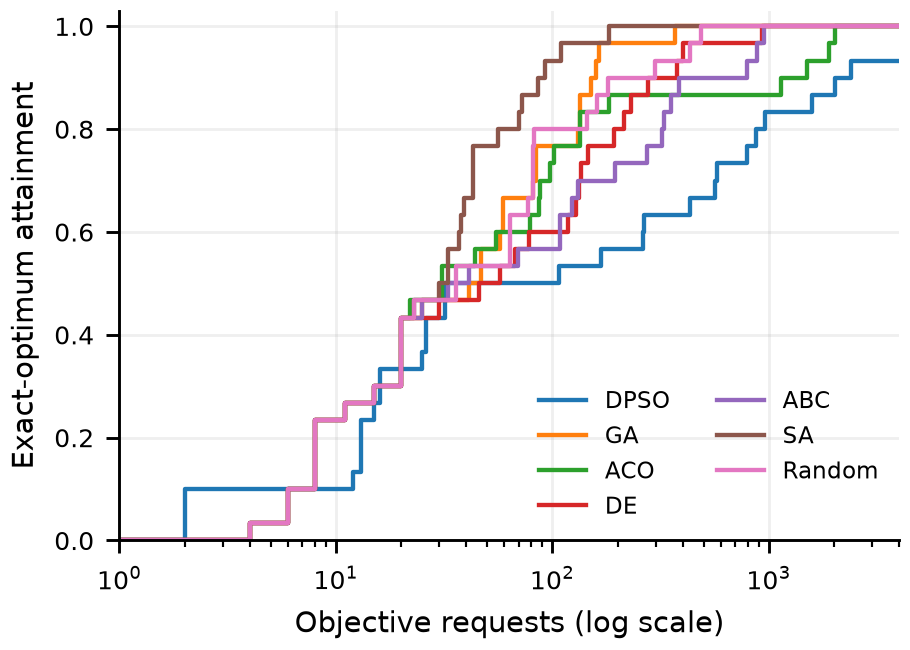
\includegraphics[width=\columnwidth]{assets/revision_attainment.png}
    \caption{Exact-optimum attainment in the unfiltered NeuMF grammar, using recorded first-hit requests. Each method has ten searches on each of three fixed checkpoints. Searches that fail to reach an optimum remain unattained at 4,000 requests.}
    \label{fig:attainment}
\end{figure}

\subsection{Feature Selection Attenuates Observed Gaps}
\begin{table}[t]
\centering
\caption{Selection audit against exhaustive full conjunctions (294 possible cells per model). Valid counts supported full cells; retained counts high-gap full cells whose selected-feature parent also exceeds 0.02. This is threshold attenuation under aggregation, not a same-grammar optimizer comparison.}
\label{tab:selection-ablation}
\small
\begin{tabular}{rrrrrr}
\toprule
Seed & Sel. & Valid & $\Delta_{sel}$ & $\Delta_{full}$ & Retained \\
\midrule
42 & 7 & 61 & 0.01495 & 0.04662 & 0/14 \\
100 & 7 & 61 & 0.01484 & 0.04378 & 0/18 \\
2026 & 14 & 61 & 0.03669 & 0.04497 & 1/15 \\
\bottomrule
\end{tabular}
\end{table}

Exact unfiltered maximum validation gaps are 0.04662, 0.04378, and 0.04497 for seeds 42, 100, and 2026. The selected maxima are smaller by 0.03166, 0.02894, and 0.00828, respectively. These differences reflect a change in expressible predicates, rather than search failure within an unchanged grammar.

More directly, the full audit finds 14, 18, and 15 supported intersections above 0.02. Mapping those cells to their selected-feature parents leaves 0, 0, and 1 parents above threshold. The corresponding high-gap full cells contain 652, 658, and 599 audit users; only 43 users in the third model belong to a high-gap full cell with an above-threshold parent. This comparison measures attenuation by aggregation, without treating threshold flags as confirmed population harms.

The ablation supplies evidence against assuming that activity-based predictive selection preserves utility-disadvantage signals. The observed reduction is determined by backward elimination from all three audit attributes. The appropriate conclusion is that the evaluated activity-proxy wrapper can conceal observed intersectional gaps, even while simplifying optimization. A practical audit should enumerate a tractable full grammar and evaluate gap retention before accepting a projected grammar; predictive activity accuracy alone is insufficient evidence of that retention.

\subsection{Selection-Target, Subset-Size, and Support Ablations}
\begin{table*}[t]
\centering
\caption{MovieLens target-by-cap ablation at support 20: exact maximum gap and, in parentheses, high full cells with an above-threshold parent divided by all high full cells. A/U denote activity/utility-deficit targets; 2/3 are maximum subset sizes. Each selection arm applies backward elimination from the complete audit schema.}
\label{tab:target-ablation}
\small
\begin{tabular}{rlllll}
\toprule
Seed & A2 & A3 & U2 & U3 & Full \\
\midrule
42 & 0.0150 (0/14) & 0.0466 (14/14) & 0.0150 (0/14) & 0.0150 (0/14) & 0.0466 (14/14) \\
100 & 0.0148 (0/18) & 0.0148 (0/18) & 0.0274 (3/18) & 0.0274 (3/18) & 0.0438 (18/18) \\
2026 & 0.0367 (1/15) & 0.0367 (1/15) & 0.0226 (1/15) & 0.0226 (1/15) & 0.0450 (15/15) \\
\bottomrule
\end{tabular}
\end{table*}

Table~\ref{tab:target-ablation} compares activity and utility-deficit targets under caps two and three. For seed 42, relaxing the activity cap retains all three attributes and all 14 above-threshold full cells, whereas utility-target selection retains age alone and none of those cells under either cap. For seed 100, utility-target selection retains occupation and preserves 3 of 18 full-cell flags, compared with none under activity selection. For seed 2026, both targets preserve only 1 of 15 flags, despite different selected grammars. A utility-related label therefore does not by itself guarantee retention of intersectional utility gaps, and a relaxed cap is not a requirement to retain every attribute.

Support sensitivity supplies a second boundary. Raising the full-grammar support threshold from 20 to 50, 100, and 200 leaves 61, 19, 8, and 1 supported cells, respectively, for each MovieLens checkpoint. The above-threshold counts change from 14/18/15 at support 20 to 6/4/4 at 50, 1/1/1 at 100, and 0/0/0 at 200. This is a change in the population intersections admitted to the audit, not evidence that higher support removes underlying harms. These controls remain post hoc and concern the specified wrapper and support policy.

\subsection{Additional Datasets: Projection and Search}
\begin{table*}[t]
\centering
\caption{Additional frozen DeepFM audits at support 20. Users are development/discovery/confirmation; cells are total/supported full conjunctions; retained counts full high-gap cells whose selected parent remains above 0.02. Selected features use development-utility labels and a two-feature cap.}
\label{tab:additional-datasets}
\small
\begin{tabular}{llrlrrr}
\toprule
Dataset & Users (D/A/C) & Full cells & Selected predicates & $\Delta_{full}$ & $\Delta_{sel}$ & Retained \\
\midrule
LFM360K & 80,110/93,461/93,463 & 53,058/894 & gender, country & 0.2511 & 0.1173 & 115/323 \\
Amazon & 52,763/61,557/61,558 & 1,000/325 & history, max price & 0.1699 & 0.0878 & 15/84 \\
\bottomrule
\end{tabular}
\end{table*}

\begin{table*}[t]
\centering
\caption{Additional datasets: exact-optimum hit rate / mean above-threshold recall (percent), ten search seeds per method/grammar at 4,000 requests. Each dataset has one supplied checkpoint; all seven methods are evaluated in both selected and full grammars.}
\label{tab:additional-search}
\small
\begin{tabular}{llrrrrrrr}
\toprule
Dataset & Space & DPSO & GA & ACO & DE & ABC & SA & Random \\
\midrule
LFM360K & Sel. & 30/51 & 100/100 & 100/99 & 30/69 & 100/89 & 100/98 & 100/100 \\
LFM360K & Full & 0/1 & 0/15 & 20/19 & 10/28 & 0/8 & 30/20 & 20/7 \\
Amazon & Sel. & 100/73 & 100/100 & 100/97 & 100/100 & 100/100 & 100/100 & 100/100 \\
Amazon & Full & 50/23 & 90/89 & 30/46 & 60/58 & 90/93 & 50/73 & 100/98 \\
\bottomrule
\end{tabular}
\end{table*}

The additional datasets test the limits of the MovieLens observation, using a different frozen model and ranking protocol (Table~\ref{tab:additional-datasets}). LFM360K's full grammar contains 53,058 cells, but only 894 meet support 20. The two-feature utility-target pipeline retains gender and country, yielding 478 possible cells and a maximum observed gap of 0.11735, compared with 0.25111 in the full grammar. Of 323 high-gap full cells, 115 retain an above-threshold projected parent. The corresponding Amazon behavioral-profile audit reduces 1,000 possible cells to 100, with maximum observed gaps 0.16988 and 0.08781; only 15 of 84 high-gap full cells retain an above-threshold parent. For both datasets, the full-size cap yields the same selected subset as cap two. These are effects of the evaluated utility-target/backward-elimination pipeline, not replications of the MovieLens activity-proxy label or evidence of protected-group disadvantage in Amazon.

Table~\ref{tab:additional-search} shows dataset-dependent search behavior. In LFM360K's selected grammar, random, GA, ACO, ABC, and SA attain every optimum; native DPSO and DE attain three of ten. In the sparse full grammar, SA attains three of ten, ACO and random two, DE one, and the other methods none. SA has the smallest descriptive mean regret (0.02308), but ten searches on one checkpoint do not establish general superiority. DE has the highest full-grammar threshold recall (27.6\%), illustrating that breadth and extreme-score attainment need not identify the same method.

In Amazon, every method attains all ten selected-grammar optima. Random sampling also attains all ten full-grammar optima with 98.0\% mean threshold recall, whereas GA and ABC attain nine of ten and native DPSO five. Thus a larger grammar alone does not establish a need for adaptation; supported density, budget relative to space size, and objective geometry also matter. Exhaustive references remain computationally feasible for all these grammars, although LFM360K enumeration uses more than the heuristic request budget.

\begin{table*}[t]
\centering
\caption{One discovery-fixed rule per additional dataset/grammar, confirmed on disjoint users. Bounds are pointwise 95\% bounded-outcome intervals, conditional on the supplied checkpoint and fixed membership proportion; no familywise guarantee is claimed.}
\label{tab:additional-confirmation}
\small
\begin{tabular}{llrrrl}
\toprule
Dataset & Space & $\Delta_D$ & $\Delta_C$ & Support & Interval \\
\midrule
LFM360K & Sel. & 0.1173 & 0.0766 & 12 & [-0.356, 0.509] \\
LFM360K & Full & 0.2511 & 0.1101 & 20 & [-0.226, 0.446] \\
Amazon & Sel. & 0.0878 & 0.0109 & 48 & [-0.209, 0.230] \\
Amazon & Full & 0.1699 & 0.1023 & 18 & [-0.252, 0.457] \\
\bottomrule
\end{tabular}
\end{table*}

The fixed LFM360K full-rule gap falls from 0.25111 in discovery to 0.11013 on separate confirmation users; its selected-rule gap falls from 0.11735 to 0.07657. Amazon's full and selected gaps change from 0.16988/0.08781 to 0.10229/0.01092. Every pointwise bounded-outcome interval includes zero (Table~\ref{tab:additional-confirmation}). These observations show attenuation and uncertain persistence under the supplied protocols; they do not confirm population discrimination or repair incomplete checkpoint provenance.

\subsection{MovieLens Test Confirmation and Uncertainty}
\begin{table}[t]
\centering
\caption{Fixed exhaustive validation maximizers on test interactions of the same audit users. Conservative pointwise bounded-outcome intervals guard against sparse-cell bootstrap degeneracy. Neither these nor the separately recorded 2,000-resample bootstrap intervals adjust for adaptive selection or provide independent-user confirmation.}
\label{tab:extended-confirmation}
\small
\begin{tabular}{rlrrrl}
\toprule
Seed & Space & N & Val. & Test & Interval \\
\midrule
42 & Sel. & 367 & 0.0150 & +0.0072 & [-0.085,+0.100] \\
42 & Full & 25 & 0.0466 & +0.0234 & [-0.294,+0.340] \\
100 & Sel. & 367 & 0.0148 & +0.0160 & [-0.076,+0.108] \\
100 & Full & 22 & 0.0438 & -0.0670 & [-0.404,+0.270] \\
2026 & Sel. & 52 & 0.0367 & -0.0594 & [-0.285,+0.166] \\
2026 & Full & 22 & 0.0450 & -0.0598 & [-0.396,+0.277] \\
\bottomrule
\end{tabular}
\end{table}

The selected-grammar maximizers are users aged 50 for model seeds 42 and 100 (367 users), and female users in age category 1 for seed 2026 (52 users). Their test gaps are 0.00722, 0.01601, and $-0.05944$, respectively. The fixed full-grammar maximizers have supports 25, 22, and 22, and test gaps 0.02338, $-0.06696$, and $-0.05983$. Full maxima tie across 2, 5, and 5 cells, respectively; enumeration order fixes one rule before confirmation. Approximately 91\% of audit users have zero validation NDCG@10. This sparse single-item utility and the presence of tied zero-hit groups limit interpretation of the maxima and their test persistence.

Validation disadvantages therefore do not consistently persist on test interactions. Conservative bounded-outcome intervals include zero for all six fixed rules. The separately recorded bootstrap intervals can be narrower, particularly in sparse cells, but neither calculation adjusts for adaptive selection, shared audit users, or the post hoc extension. These results establish observed validation differences and uncertainty about persistence, rather than confirmed discriminatory treatment.

\subsection{Expanded Behavioral Auditing}
\begin{table}[t]
\centering
\caption{Companion measurements for GA-selected subgroups, averaged equally across three model seeds. Gaps are group minus global; a negative diversity gap denotes lower diversity.}
\label{tab:audit}
\small
\begin{tabular}{llrrr}
\toprule
Measurement & Split & Group & Global & Gap \\
\midrule
Calibration (JSD) & Val. & 0.16646 & 0.16853 & -0.00208 \\
 & Test & 0.16662 & 0.16861 & -0.00199 \\
Exposure (TV) & Val. & 0.51512 & 0.49630 & +0.01882 \\
 & Test & 0.51498 & 0.49611 & +0.01887 \\
Intra-list diversity & Val. & 0.57709 & 0.60205 & -0.02495 \\
 & Test & 0.57724 & 0.60236 & -0.02513 \\
\bottomrule
\end{tabular}
\end{table}

For the original GA-selected subgroups, validation calibration divergence averages 0.16646 versus 0.16853 globally, a signed gap of $-0.00208$. Exposure-opportunity mismatch averages 0.51512 versus 0.49630, a gap of $+0.01882$. Intra-list diversity averages 0.57709 versus 0.60205, a gap of $-0.02495$. These are equal-weight means across three model seeds, not pooled user means. Within each original seed, the other search methods select the same subgroup and yield the same companion measurements.

Calibration gaps vary in sign across seeds, whereas exposure-opportunity mismatch is higher and intra-list diversity lower in each selected subgroup. These descriptive measurements contextualize utility differences; they do not establish significance or causal harm. Their interpretation depends on the declared eligible-catalog opportunity reference~\cite{burke2017multisided,biega2018equity,singh2018fairness}. The extension's utility-only search timings exclude these companion aggregations and are not pooled with the original timings.
